% Use the lineno option to display guide line numbers if required.
\documentclass[9pt,twocolumn,twoside,lineno]{pnas-new}

\usepackage{enumitem,listings}

% Automatic formatting of SI units
\usepackage[binary-units]{siunitx}

% Set options for code listings
\lstset{language=C++}

% Turn off whitespace around lists
\setlist{nolistsep}

% Visible TODO notes
\newcommand{\todo}[1]{\textbf{\textsc{\textcolor{red}{(TODO: #1)}}}}

\templatetype{pnasresearcharticle} % Choose template 
% {pnasresearcharticle} = Template for a two-column research article
% {pnasmathematics} %= Template for a one-column mathematics article
% {pnasinvited} %= Template for a PNAS invited submission

\title{Large-scale brain simulations on the desktop using procedural connectivity}

% Use letters for affiliations, numbers to show equal authorship (if applicable) and to indicate the corresponding author
\author[a,1]{James C Knight}
\author[a]{Thomas Nowotny} 

\affil[a]{Centre for Computational Neuroscience and Robotics, School of Engineering and Informatics, University of Sussex, Brighton, United Kingdom}

% Please give the surname of the lead author for the running footer
\leadauthor{Knight} 

% Please add here a significance statement to explain the relevance of your work
\significancestatement{Authors must submit a 120-word maximum statement about the significance of their research paper written at a level understandable to an undergraduate educated scientist outside their field of speciality. The primary goal of the Significance Statement is to explain the relevance of the work in broad context to a broad readership. The Significance Statement appears in the paper itself and is required for all research papers.}

% Please include corresponding author, author contribution and author declaration information
\authorcontributions{J.K. and T.N. wrote the paper.
T.N. is the original developer of GeNN.
J.K. is currently the primary GeNN developer and was responsible for extending the code generation approach to the procedural simulation of synaptic connectivity.
J.K. performed the experiments and the analysis of the results that are presented in this work.}

\authordeclaration{The authors declare no conflict of interest.}
\correspondingauthor{\textsuperscript{1}To whom correspondence should be addressed. E-mail: J.C.Knight\@sussex.ac.uk}

% Keywords are not mandatory, but authors are strongly encouraged to provide them. If provided, please include two to five keywords, separated by the pipe symbol, e.g:
\keywords{spiking neural networks $|$ GPU $|$ high-performance computing $|$ brain simulation} 

\begin{abstract}
Large-scale simulations of spiking neural networks are important for improving our understanding of the dynamics and ultimately function of brains.
However, even small mammals such as mice have approximately \num{1E12} synaptic connections which are typically charaterized by at least one floating point value per synapse.
This amounts to several terabytes of connection data -- an unrealistic memory requirement for a single desktop machine.
Simulations of large spiking neural networks are therefore typically executed on large distributed supercomputers.
This is costly and limits large-scale modelling to a select few research groups with the appropriate resources.
%However, large parts of current brain models are described by simple algorithms which determine the existence and conductance of synaptic connections. 
In this work, we describe extensions to GeNN -- our GPU-based spiking neural network simulator -- that enable it to `procedurally' generate connectivity and synaptic weights `on the go' as spikes are triggered, instead of storing and retrieving them from memory.
We find that GPUs are well-suited to this approach because of their raw computational power, which due to memory bandwidth limitations is often under-utilised when simulating spiking neural networks.
We demonstrate the value of our approach with a recent model of the Macaque visual cortex consisting of \num{4.13E6} neurons and \num{24.2E9} synapses.
Using our new method, this model can be simulated on a single GPU.
Our results match those obtained on a supercomputer and the simulation runs faster on a single high-end GPU than a previous simulation executed on over 1000 supercomputer nodes.
\end{abstract}

\dates{This manuscript was compiled on \today}
\doi{\url{www.pnas.org/cgi/doi/10.1073/pnas.XXXXXXXXXX}}

\begin{document}

\maketitle
\thispagestyle{firststyle}
\ifthenelse{\boolean{shortarticle}}{\ifthenelse{\boolean{singlecolumn}}{\abscontentformatted}{\abscontent}}{}

\dropcap{T}he brain of a mouse has around \num{70E6} neurons, but this number is dwarfed by the \num{1E12}~\citep{Herculano-Houzel2010} synapses which connect them.
%While simulating synaptic plasticity -- the family of mechanisms believed to be %responsible for learning -- represents a further challenge, in a large-scale model, it is unlikely that learning would be enabled on \emph{all} synapses so efficiently simulating the remaining static synapses is a key challenge for large-scale brain simulation.\todo{has this been at all quantified in mice?}
In computer simulations of spiking neural networks, propagating spikes through synapses involves reading a `row' of synapses connecting a spiking presynaptic neuron to its postsynaptic partners and adding the `weight' of each synapse in the row to a `bin' containing the postsynatic neuron's input for the next simulation timestep.
%Because typical EPSP shaping functions are linear, they can then be subsequently applied to the `histogram' resulting from this process.~\todo{presumably someone first had this intuition so cite}.
Typically, the information describing which neurons are connected by a synapse and with what conductance, is generated before a simulation is run and stored in large matrices in random access memory~(RAM). 
This creates high memory requirements for large-scale brain models, so that they can typically only be simulated on large distributed computer systems using software such as NEST~\citep{Gewaltig2007} or NEURON~\citep{carnevale2006neuron}.
By careful design, these simulators can keep the memory requirements for each node constant, even when a simulation is distributed across thousands of nodes~\citep{Jordan2018}.
However, high performance computer systems are bulky, expensive and consume large amounts of power, meaning that they are typically shared resources that are only accessible to a limited number of researchers and for strongly time-limited investigations.

Neuromorphic systems~\citep{Frenkel2018,Frenkel2019,Furber2014,Merolla2014,Qiao2015,Schemmel2017} take inspiration from the brain and have been developed specifically for simulating large spiking neural networks.
One particular relevant feature of the brain is that its memory elements -- the synapses -- are co-located with the computing elements -- the neurons -- throughout the entire system.
In neuromorphic systems, this often translates to dedicating a large proportion of each chip to memory.
However, while such on-chip memory is fast, it can only be fabricated at relatively low density meaning that many of these systems economize -- either by reducing the maximum number of synapses per neuron to as few as \num{256} or by reducing the precision of the synaptic weights to \num{6}~\citep{Schemmel2017}, \num{4}~\citep{Frenkel2018} or even \SI{1}{\bit}~\citep{Merolla2014,Frenkel2019}.
Such strategies allow some classes of spiking neural networks to be simulated very efficiently, but reducing the degree of connectivity in large-scale brain simulations to fit within the constraints of current neuromorphic systems inevitably changes their dynamics~\citep{VanAlbada2015}.
Unlike the majority of other neuromorphic systems, the SpiNNaker~\citep{Furber2014} neuromorphic super-computer is entirely programmable and combines a large amount of on-chip memory with external memories, distributed across the system for the storage of synaptic connectivity.
SpiNNaker's external memory bandwidth, on-chip memory capacity and the computational power of each core are all tailored to large-scale brain simulation meaning that the output bins of the synapse processing algorithm can fit in on-chip memory and there is enough external memory bandwidth to fetch synaptic rows fast enough for real-time simulation of large-scale models~\citep{Rhodes2019}.
This is a promising approach for future research but, because of its prototype nature, the availability of SpiNNaker hardware is limited and a physically large system is still required for even moderately-sized simulations (9 boards for a simulation with around \num{10E3} neurons and \num{300E6} synapses~\citep{Rhodes2019}).
%However, a physically large system is required for even moderately-sized simulations (9 boards for a simulation with around \num{10E3} neurons and \num{300E6} synapses~\citep{Rhodes2019})
%A next generation SpiNNaker system is currently under development~\citep{Mayr2019} and, by employing a newer fabrication technology (\SI{22}{\nano\meter} rather than \SI{130}{\nano\meter}), a single chip of the new system will offer equivalent performance to 48 of the current chips.
%Nonetheless, large-scale brain simulations will still require a large multi-chip system.

Modern GPUs have relatively small amounts of on-chip memory and, instead, dedicate the majority of their silicon area to arithmetic logic units~(ALUs).
GPUs use dedictated hardware to rapidly switch between tasks so that the latency of accessing external memory can be `hidden' behind computation, as long as there is sufficient computation to be performed.
For example, the memory latency of a typical modern GPU can be completely hidden if each CUDA core performs approximately 10 arithmetic operations per byte of data accessed from memory.
Unfortunately, processing a synapse in a spiking neural network simulation is likely to require accessing approximately \SI{8}{\byte} of memory and performing many fewer than the required 80 instructions. This makes synaptic updates highly memory bound.
Nonetheless, we have shown in previous work~\citep{Knight2018} that, as GPUs have significantly higher total memory bandwidth than even the most expensive CPU, moderately sized models of around \num{10E3} neurons and \num{1E9} synapses can be simulated on a single GPU with competitive speed and energy requirements.
However, individual GPUs do not have enough memory to simulate truly large-scale brain models and, although small numbers of GPUs can be connected together using the high-speed NVLink~\todo{cite} interconnect, beyond such small GPU clusters, scaling will be dictated by the same communication overheads as for other MPI-based distributed systems.

In this work we present a novel approach which converts large-scale brain simulation from a problem which is memory-bound on a GPU to one where the large amount of computational power available on a GPU can be used to reduce both memory and memory bandwidth requirements and enable truly large-scale brain simulations on a single GPU workstation.

\begin{figure*}
    \centering
    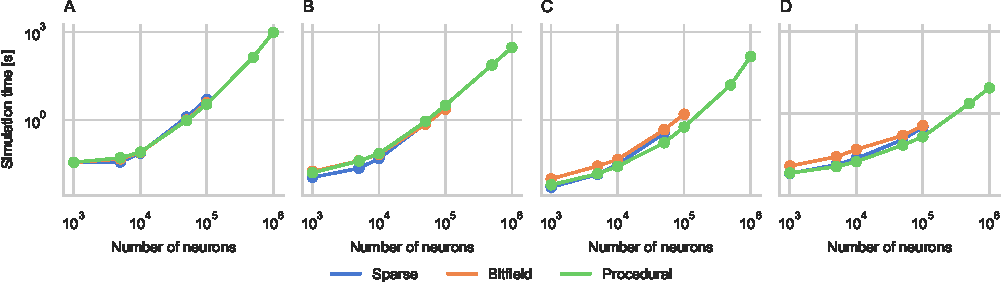
\includegraphics{figures/performance_scaling}
    \caption{Simulation time performance scaling on a range of modern GPUs (colors). \textbf{A} The best performing approach at each scale on each GPU (indicated by the symbols). For the largest models, the procedural method is always best.
    \textbf{B} Raw performance of each approach on each GPU.
    Missing bars indicate insufficient memory to simulate.}
    \label{fig:performance_scaling}
\end{figure*}

\section*{Results}
In the following subsections, we will first present two recent innovations in our GeNN simulator~\citep{Yavuz2016} which allow it to be used for simulating large-scale models on a single GPU.
We will then demonstrate the power of these new features by simulating a recent model of the Macaque visual cortex~\citep{Schmidt2018} consisting of \num{4.13E6} neurons and \num{24.2E9} synapses on a single GPU.
We find that we not only obtain the same results as in the previous simulation on a high-performance supercomputer, but our simulation also runs faster.

\subsection*{Procedural connectivity}
Our GeNN simulator~\citep{Yavuz2016} uses code generation to convert neuron and synapse models -- described using `snippets' of C-like code -- into CUDA code for GPU simulation.
We previously extended GeNN to allow the same approach to be used for generating efficient, parallel model initialisation code from code snippets describing state variable and synaptic connectivity initialisation algorithms~\citep{Knight2018}.
Offloading initialisation to the GPU sped up model initialisation by around $20\times$ on a desktop PC~\citep{Knight2018}, suggesting that these initialisation algorithms are well-suited to GPU acceleration.
\todo{something explaining why this is for synapses}
In fact, it seems somewhat illogical to run these algorithms only once to fill the limited memory of the GPU with data only to then read it back throughout the simulation and in so doing, overload the limited memory bandwidth.

What if we could instead `procedurally' generate connectivity and synaptic weights `on the go' as spikes are triggered?
If we could do this in less than than the 80 instructions required to hide the memory latency in the current approach, this new approach could be \emph{faster} as well as requiring no memory to story connectivity and synaptic weights.
Although this idea has not been previously applied to modern hardware, Eugene Izhivich used a similar approach for simulating an extremely large thalamo-cortical model with \num{1E11} neurons and \num{1E15} synapses on a modest PC cluster in 2005~\todo{cite}.
Sadly, while this remains an incredible achievement, simulating the model for 1 second of biological time required 50 days of simulation.
However, high-end GPUs have thousands of times more compute power than the CPUs available in 2005 and, due to the limited memory bandwidth available to each of their parallel computing elements, are particularly well-suited to this approach.

\begin{figure*}
    \centering
    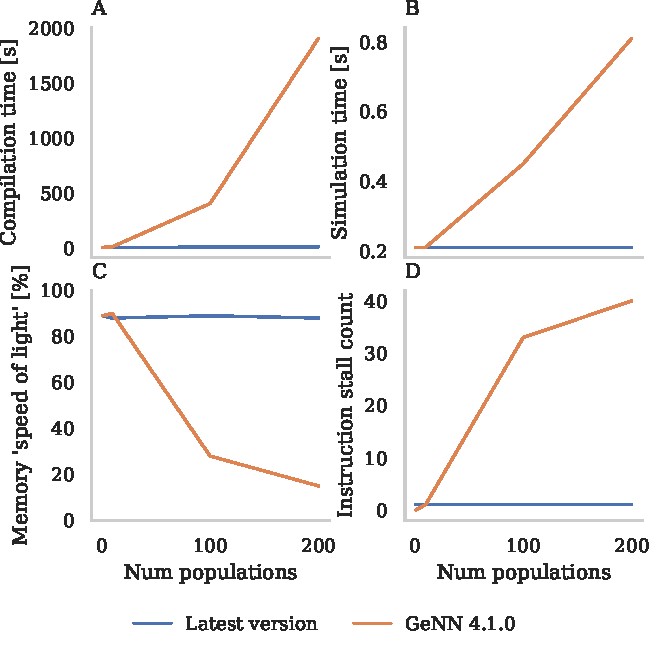
\includegraphics{figures/merging_scaling}
    \caption{Performance of a simulation of \num{1000000} LIF neurons driven by a gaussian input current, partitioned into varying numbers of populations and running on a workstation equipped with a Titan RTX GPU.
    \textbf{A} Compilation time using GCC 7.5.0.
    \textbf{B} Simulation time for an \SI{1}{\second} simulation.
    \textbf{C} Memory throughput reported by NVIDIA Nsight compute profiler 'Speed of light' metric.
    \textbf{D} Number of 'No instruction' stalls reported by NVIDIA Nsight compute profiler.}
    \label{fig:merging_scaling}
\end{figure*}

To demonstrate the performance and scalability of our `procedurally' generate connectivity, we used a network, initially designed as a medium for experimentation into signal propagation through cortical networks~\citep{Vogels2005}, but subsequently widely used as a scalable benchmark~\citep{Brette2007}.
The network consists of $N$ integrate-and-fire neurons, partitioned into $\frac{4N}{5}$ excitatory and $\frac{N}{5}$ inhibitory neurons.
The populations are connected all-to-all with a fixed $P_{\text{conn}}=\SI{10}{\percent}$ probability of a synapse existing between a pair of neurons, meaning that the postsynaptic targets of a presynaptic neuron can be modelled using a Bernoulli distribution $\text{Bern}[P_{\text{conn}}]$.
The Bernoulli distribution can be sampled by repeatedly drawing from the uniform distribution $\text{Unif}[0, 1]$ and comparing each sample to $P_{\text{conn}}$, but this is innefficient for sparse connectivity.
Instead we can sample from the geometric distribution $\text{Geom}[P_{\text{conn}}]$ which describes how the number of Bernoulli trials required to get a success (i.e. a synapse) is distributed.
The geometric distribution can be sampled in constant time by inverting the cumulative density function~(CDF) of the equivalent continuous distribution (the exponential distribution) to obtain $\frac{log(\text{Unif}[0, 1])}{log(1 - P_{\text{conn}})}$~\citep[p499]{DevroyeLuc2013}.
Therefore, as long as one has the ability to generate a unique but repeatable stream of random numbers for each presynaptic neuron, the postsynaptic targets of a presynaptic neuron can be `procedurally' generated  in parallel.
While suitable random number streams \emph{could} be provided by a `convential' random number generator~(RNG), each presynaptic neurons would need to maintain its own RNG state which would have a significant memory overhead.
Instead, we use a `counter-based' Philox4$\times$32-10 RNG~\citep{Salmon2011}.
Counter-based RNGs are designed for parallel applications and essentially consist of a pseudo-random bijective function which takes a counter as an input (in this case a \SI{128}{\bit} number) and outputs random numbers.
In constrast to convential RNGs, this means that generating the $n^\text{th}$ random number in a stream has exactly the same cost as generating the `next' random number, allowing us to trivially to divide up the random number stream between multiple parallel processes (in this case presynaptic neurons).
\todo{do we need some more explanation of how you get from this to a network simulation?}

We ran simulations of this network at scales ranging from \num{1E3} to \num{1E6} neurons (corresponding to ~\num{100E3} and \num{100E9} synapses respectively) on a selection of modern NVIDIA GPU hardware:
%
\begin{description}[noitemsep]
    \item [Jetson TX2] a low-power embedded system designed for robotic applications with \SI{8}{\giga\byte} of shared memory
    \item [Geforce MX130] a laptop GPU with \SI{2}{\giga\byte} of dedicated memory
    \item [Geforce GTX 1650] a low-end desktop GPU with \SI{4}{\giga\byte} of dedicated memory
    \item [Titan RTX] a high-end workstation GPU with \SI{24}{\giga\byte} of dedicated memory
\end{description}
%
In Fig.~\ref{fig:performance_scaling} we compare the duration of these simulations using our new procedural approach against the standard approach of storing synaptic connections in memory using two different data structures.
Both data structures are described in more detail in our previous work~\citep{Knight2018} but briefly, in the `sparse' data structure, a presynaptic neuron's postsynaptic targets are represented as a sorted array of indices whereas, in the `bitfield' data structure, they are represented as `1s' in a bitfield with a bit for each postsynaptic neuron.
None of the devices have enough memory to store the \num{100E9} synapses required for the largest scale using either data structure but, at the \num{100E3} neuron scale, the bitfield data structure allows the model to fit into the memory of several devices it otherwise would not.
However, not only is the new procedural approach the \emph{only} way of simulating models at the largest scales but, as Fig.~\ref{fig:performance_scaling} illustrates, even at smaller scales its performance is competitive with and sometime better than the standard approach.
\todo{note that this is using synapses with fixed synaptic weight}

\subsection*{Kernel merging}
While the procedural connectivity approach presented in the previous section allows us to simulate models which would otherwise not fit within the memory of a single GPU, there are additional problems when using code generation to generate simulation code for models with large numbers of neuron and synapse populations.

GeNN and -- to the best of our knowledge~\citep{Blundell2018} -- all other SNN simulators which use code generation to generate all of their simulation code (as opposed to, for example NESTML~\citep{Plotnikov2016}, which uses code generation to generate neuron simulation code) generate seperate pieces of code to simulate each population of neurons and synapses.
This approach allows optimizations such as the hard-coding of constant parameters to be easily performed and, although generating code for models with many populations will result in large code size, C++ CPU code  can be easily divided between multiple modules and compiled in parallel, minimizing the effect on build time.
However, GPUs can only run a small number of kernels -- which are equivalent to modules in this context --  simultaneously (128 on the latest NVIDIA GPUs~\todo{cite}).
Therefore, in GeNN, multiple neuron populations are simulated within each kernel, resulting in code of the form shown in the following pseudocode which illustrates how 3 populations of 1000 neurons could be simulated in a single kernel:
\todo{very minimal sentance about SIMT here}

\begin{lstlisting}
void updateNeurons()
{
  if(thread < 1000) {
    // Update neuron population A
  }
  else if(thread >= 1000 && thread < 2000) {
    // Update neuron population B
  }
  else if(thread >= 2000 && thread < 3000) {
    // Update neuron population C
  }
}

\end{lstlisting}

\begin{figure*}
    \centering
    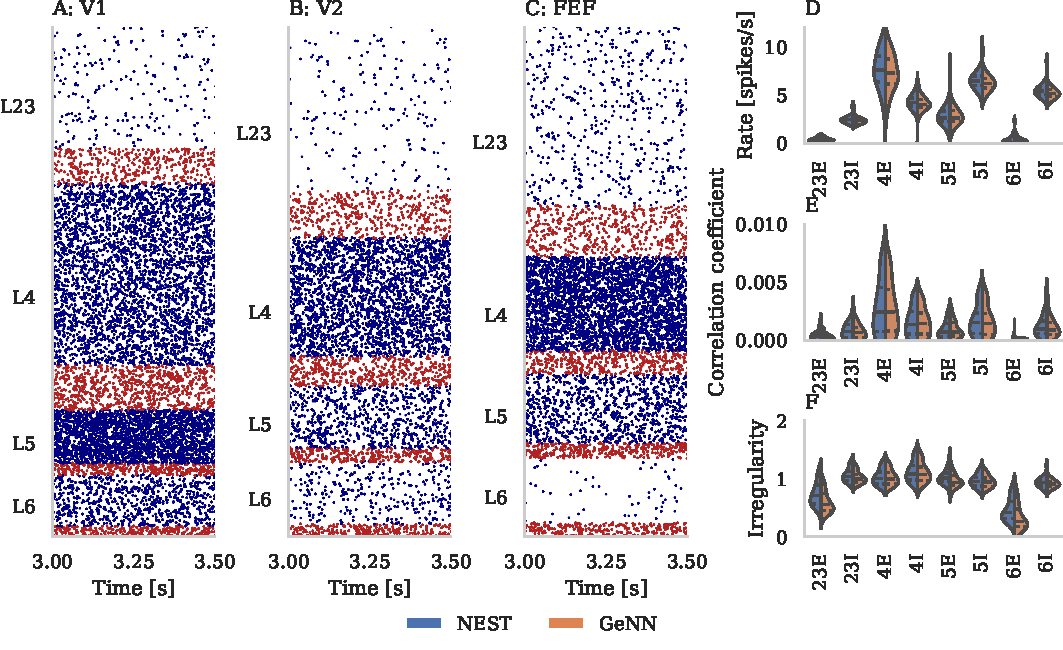
\includegraphics{figures/multi_area}
    \caption{Results of full-scale multi-area model simulation. 
    \textbf{A-C} Raster plots of spiking activity of \SI{3}{\percent} of the neurons in area V1~\textbf{A}, V2~\textbf{B}, and FEF~\textbf{C}. 
    Blue: excitatory neurons, red: inhibitory neurons.
    \textbf{D-F} Spiking statistics for each population across all 32 areas simulated using GeNN and NEST shown as split violin plots.
    Solid lines: medians, Dashed lines: Interquartile range~(IQR).
    \textbf{D} Population-averaged firing rates.
    \textbf{E} Average pairwise correlation coefficients ofspiking activity. 
    \textbf{F} Irregularity measured by revised local variation LvR~\citep{Shinomoto2009} averaged across neurons.}
    \label{fig:multi_area}
\end{figure*}

This approach works well for models with small numbers of populations but, as Fig.~\ref{fig:merging_scaling}A illustrates, when we partition a model consisting of \num{1000000} LIF neurons into a large number of populations (increasing the size of the neuron kernel), compilation times increases super-linearly -- quickly becoming impractical.
Furthermore, Fig.~\ref{fig:merging_scaling}B shows that when the model is partitioned into a large number of populations, the simulation also runs much more slowly.
We would expect this model to be memory bound as each thread in the model reads \SI{32}{\byte} of data and, as we discussed previously, hiding the latency of these memory accesses would require approximately 320 arithmetic operations which is many more than are required to sample from the uniform distribution and update a LIF neuron.
Fig.~\ref{fig:merging_scaling}C -- obtained using data from the NVIDIA Nsight compute profiler~\todo{cite} -- shows that this to be true with the memory system being around \SI{90}{\percent} utilised for small numbers of populations.
However, when the model is partitioned into large numbers of populations, the kernel stops being able to efficiently use the memory and become latency bound (neither memory \emph{or} compute are used efficiently).
Investigating further using the profiler showed that this drop in performance was accompanied by an increasing number of ``No instruction'' stalls as shown in Fig.~\ref{fig:merging_scaling}D.
Stalls are events which prevent the GPU from doing any work during a clock cycle and the profiler documentation suggests that these particular events are likely to be caused by ``Excessively jumping across large blocks of assembly code''\todo{cite} -- which makes sense when we are generating kernels with hundreds of thousands of lines of code.
\todo{is more detail required here as to why?}

To address these issues, we developed a new code generator for GeNN which first `merges' the model description, grouping populations which can be simulated using the same generated code.
From this merged description, structures are generated to store the pointers to state variables and the parameters which differ between merged populations:
%
\begin{lstlisting}
struct NeuronUpdateGroup
{
  unsigned int numNeurons;
  float* V;  
};

\end{lstlisting}
%
An array of these structures is then declared for each merged population and each element is initialised with pointers to state variables and parameter values:
%
\begin{lstlisting}
NeuronUpdateGroup neuronUpdateGroup[3];
neuronUpdateGroup[0] = {1000, VA};
neuronUpdateGroup[1] = {1000, VB};
neuronUpdateGroup[2] = {1000, VC};
\end{lstlisting}
%
In order for a thread to determine which neuron in which population it should be simulating, we generate an additional data structure -- an array containing a cumulative sum of threads used for each population.
Each thread performs a simple binary search within this to find the index of the neuron and population it should simulate:
%
\begin{lstlisting}
unsigned int startThread[3] = {0, 1000, 2000};
void updateNeurons()
{
  if(thread < 3000) {
    // Binary search startThread to determing
    // which population thread should be 
    // processed. Then update using variables 
    // in neuronUpdateGroup
  }
}
\end{lstlisting}
%
As Fig.~\ref{fig:merging_scaling} shows, this approach entirely solves the issues with compilation time and simulation performance caused by large numbers of populations.
Therefore, we apply this approach to initialisation and simulation kernels for both neuron and synapse populations.

\subsection*{The multi-area model}
Due to lack of computing power and insufficiently detailed connectivity data, previous models of the cortex have either focussed on modelling individual local microcircuits at the level of individual cells~\citep{Izhikevich2008,Potjans2012} or modelling multiple connected areas at a higher level of abstraction where entire ensembles of neurons are described by a small number of differential equations~\todo{find citation}.
However, data from several species has shown that cortical activity has distinct features at both the global and local levels which can only be captured by modelling interconnected microcircuits at the level of individual cells~\todo{find citation}.
The multi-area model~\citep{Schmidt2018a,Schmidt2018} does just this -- using scaled versions of a previous 4 layer microcircuit model~\citep{Potjans2012} to implement \SI{1}{\milli\meter\squared} `patches' for 32 areas of the macaque cortex involved in visual processing.
The 32 areas are connected together with connectivity based on inter-area axon tracing data from the CoCoMac~\citep{Bakker2012} database, refined using additional anatomical data~\citep{Markov2014} and heuristics~\citep{Ercsey-Ravasz2013} to obtain estimates for the number of synapses connecting pairs of areas.
Synapses between areas are then distributed between the populations which make up each area \todo{finish}
This model was simulated using NEST~\citep{Gewaltig2007} on a single rack~(a \SI{2}{\metre} high enclosure containing \num{1024} compute nodes and weighing over \SI{2}{\tonne}) of a IBM Blue Gene/Q supercomputer~\citep{Schmidt2018}.
On this system, initialization of the model took around \SI{5}{\minute} and simulating \SI{1}{\second} of biological time took approximately~\SI{12}{\minute}.

The multi-area model consists of \num{4.13E6} neurons split into \num{254} populations and \num{24.2E9} synapses split into \num{64516} populations meaning that, without the kernel merging approach presented earlier in this work, the model would be unlikely to compile or simulate at a reasonable speed using GeNN.
Additionally, each synapse in this model has an independant weight and synaptic delay sampled from a normal distribution, meaning that the bitfield data structure cannot be used to represent the connectivity.
Even if we assume that \SI{16}{\bit} floating point would provide sufficient weight precision, delays can be expressed as a \SI{8}{\bit} integer and that the neuron populations are all small enough to index using \SI{16}{\bit} indices, our sparse data structure would still require \SI{5}{\byte} per synapse, meaning that this model's synaptic data would require over \SI{100}{\giga\byte}.
While a cluster of GPUs connected using NVLink could be built with this much memory, it is more than any single GPU has available.

In this model the density of the synaptic connections between a pair of neuronal populations is specified in terms of a total number of random synapses~($N_{\text{syn}}$).
In order to use our procedural approach to simulate a model with this connectivity, the subset of the $N_{\text{syn}}$ synapses which end up in each row must be pre-calcualted by sampling from the multinomial distribution $\text{Mult}[N_{\text{pre}} * N_{\text{post}}, \{P_{row}, P_{row}, \ldots, P_{row}\}]$ where $P_{row} = \frac{N_{\text{post}}}{N_{\text{syn}}}$.
This operation cannot be efficiently parallelised so must be performed on the host but, once the length of each row is determined, the postsynaptic targets  of each presynaptic neuron can be `procedurally' generated  in parallel by sampling from the discrete uniform distribution $\text{Unif}[0, N_{\text{post}}]$.
% While this works mathematically, in order to improve the locality of memory accesses, synapses should be sorted into ascending order.
% This would be trivial to implement in CPU code but, without enough shared memory for each CUDA thread to store a copy of its corresponding row, an in-place sort in global memory would be very slow.
% It would be possible to use a more complex parallel sorting algorithm such as that proposed by \citet{Awan2016} but, as GPU architectures typically have very high floating point maths throughput, we instead take an alternative approach.
% Rather than sampling directly from $\text{Unif}[0, N_{\text{post}}]$ we sample from its 1st order statistic -- $\text{Beta}[1, N_{\text{post}}]$ -- essentially the next smallest value.
% In general, the Beta distribution cannot be sampled from in constant time.
% However, if $X \sim \text{Beta}[1, N_{\text{post}}]$, $1 - X \sim \text{Beta}[N_{\text{post}}, 1]$ and therefore $-ln(1 - X) \sim \text{Exponential}[N_{\text{post}}]$ -- a much simpler problem as the exponential distribution can be sampled in constant time using the inversion method~\citep[p29]{DevroyeLuc2013}.


\section*{Discussion}
\begin{itemize}
    \item Further scaling - memory only required for neuron parameters
    \item Learning
    \item Hardware for procedural connectivity?
\end{itemize}


\matmethods{Please describe your materials and methods here. This can be more than one paragraph, and may contain subsections and equations as required. Authors should include a statement in the methods section describing how readers will be able to access the data in the paper. 
\begin{itemize}
    \item LIF neuron
    \item Exponential static synapses
    \item Connectivity
    \item Parameter values for scaling and merging experiments
\end{itemize}
\subsection*{Neuron models}
The membrane voltage ($V_{j}$) of each neuron is modelled as a leaky integrate-and-fire~(LIF) unit:
%
\begin{align}
    \tau_{m} \frac{dV_{j}}{dt} = & (V_{j} - V_{rest}) + R_{m} I_{{in}_{j}} \label{eq:lif_neuron}
\end{align}
%
where $\tau_{m}$ and $R_{m}$ represent the time constant and resistance of the neuron's cell membrane, $V_{rest}$ defines the membrane voltage the neuron returns to if it receives no synaptic input and $I_{{in}_{j}}$ represents the input current to the neuron.
When the membrane voltage crosses a threshold~($V_{thresh}$) a spike is emitted, the membrane voltage is reset back to $V_{rest}$ and a countdown timer is started which, while running, disables the integration of further input thus providing a simulated refractory period.
Incoming spikes induce an exponentially-shaped input current in $I_{{in}_{j}}$:
%
\begin{align}
    \tau_{syn} \frac{dI_{{in}_{j}}}{dt} = & -I_{{in}_{j}} + I_{p_{j}} + \sum_{i=0}^{n} w_{ij} \sum_{t_{i}^{f}}  \delta(t - t_{i}^{f})\label{eq:exp_neuron_input_current}
\end{align}
%
where $\tau_{syn}$ represents the time constant with which any spikes (modelled as Dirac delta functions $\delta$) from $n$ presynaptic input neurons occuring at time $t$ are integrated.
In addition to its synaptic input, each neuron in the network also receives an independent Poisson input current $I_{p_{j}}$ (also exponentially shaped by equation~\ref{eq:exp_neuron_input_current}) which represents input from adjacent cortical regions.
}

\showmatmethods{} % Display the Materials and Methods section

\acknow{Please include your acknowledgments here, set in a single paragraph. Please do not include any acknowledgments in the Supporting Information, or anywhere else in the manuscript.}

\showacknow{} % Display the acknowledgments section

% Bibliography
\bibliography{procedural}

\end{document}
